\documentclass[tikz,border=10pt]{standalone}
\usetikzlibrary{positioning, arrows.meta, decorations.pathreplacing, calc, shapes.geometric}

\begin{document}
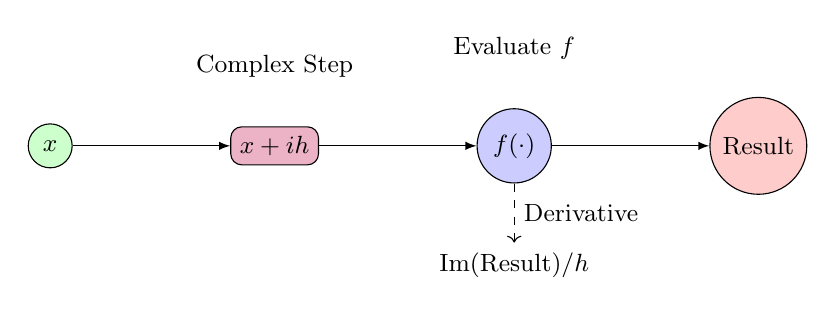
\begin{tikzpicture}[
    node distance=2cm and 2cm,
    operation/.style={circle, draw, fill=blue!20},
    input/.style={circle, draw, fill=green!20},
    output/.style={circle, draw, fill=red!20},
    complex/.style={rectangle, draw, rounded corners, fill=purple!30},
    auto/.style={->, >=latex},
    every node/.style={font=\small}
]

% Nodes
\node[input] (x) {$x$};
\node[complex, right=of x] (complexStep) {$x + ih$};
\node[operation, right=of complexStep] (f) {$f(\cdot)$};
\node[output, right=of f] (result) {Result};

% Edges
\draw[auto] (x) -- (complexStep);
\draw[auto] (complexStep) -- (f) node[midway, above] {};
\draw[auto] (f) -- (result) node[midway, above] {};

% Imaginary extraction
\node[below=0.75cm of f] (imaginary) {Im(Result)/$h$};
\draw[->, dashed] (f) -- (imaginary) node[midway, right] {Derivative};

% Annotations
\node[above=0.5cm of complexStep] (step) {Complex Step};
\node[above=0.5cm of f] (evaluate) {Evaluate $f$};

\end{tikzpicture}
\end{document}
